\documentclass{article}
\usepackage[spanish]{babel}
\usepackage{graphicx}
\usepackage{xcolor}
\usepackage[utf8]{inputenc}
\usepackage{fancyhdr}
\usepackage{lastpage}
\usepackage{enumitem}
\usepackage{listings}
\usepackage{float}

\pagestyle{fancy}
\fancyhf{}
\rfoot{Page \thepage\hspace{1pt} de~\pageref{LastPage}}

\title{Practica 2}
\author{Guillermo Lopez Garcia}
\begin{document}

\textbf{1º Parte. Despliegue del servidor apache2 y relacionados.}\\
En esta primera parte, creo el servidor apache2 y creo un programa
en PHP funcionando sobre el.\\
\\
En este programa, solo existen dos rutas posibles. Que exista en los
parametros GET la variable `save\_to\_db' o no. Es caso de que exista,
guarda el valor de la variable en un base de datos PostgreSQL\@. En caso
contrario, el programa da la información para mandar un email
automatizado desde el programa mule.\\
\\
He aquí el código PHP que ha hecho posible tal acción:\\

\lstset{language=PHP, texcl=true}
\begin{lstlisting}[frame=single]
    <?php

    // La version de php usada es la 7.2
    // y la version de apache es la 2.4

    if(isset($_GET['save_to_db']))
    {
        $host = "localhost";
        $port = "5432";
        $dbname = "sd";
        $userdb = ""; // "usuario";
        $passdb = ""; // "usuario";
        $con = pg_connect(
            " host=$host port=$port ".
            " dbname=$dbname ".
            " user=$userdb password=$passdb"
        );
        pg_insert($con, "conexiones", array(
            `email' => $_GET['save_to_db']
        ));
        pg_close($con);
    } else
    {
        echo json_encode(
            array(
                `info' => array(
                    `fromEmail'        => `',
                 // `torvalds.es.dios@gmail.com',
                    `email'            => `',
                 // `hazme.tuyo.torvalds@gmail.com',
                    `claveAplicacion'  => `',
                 // `me gusta el linux, un poco',
                    `method'           => `db'
                )
            )
        );
    }
\end{lstlisting}

También, la sentencias SQL que han hecho posible la
inyección de los datos en la base de datos PostgreSQL:\\

\lstset{language=SQL, texcl=true}
\begin{lstlisting}[frame=single]
    -- La base de datos utilizada es PostgreSQL
    -- Te preguntaras, ¿Por que PostgreSQL? ¿Tambien esta MySQL no?
    -- Y es correcto, pero yo solo uso calidad
    
    create table conexiones(
        email varchar(500),
        fecha timestamp default current_timestamp
    );
\end{lstlisting}

\textbf{2º Parte. Creación del flow de la practica en mule.}\\
A continuación, muestro una imagen del flow final de la práctica:\\
\begin{figure}[H]
\centering
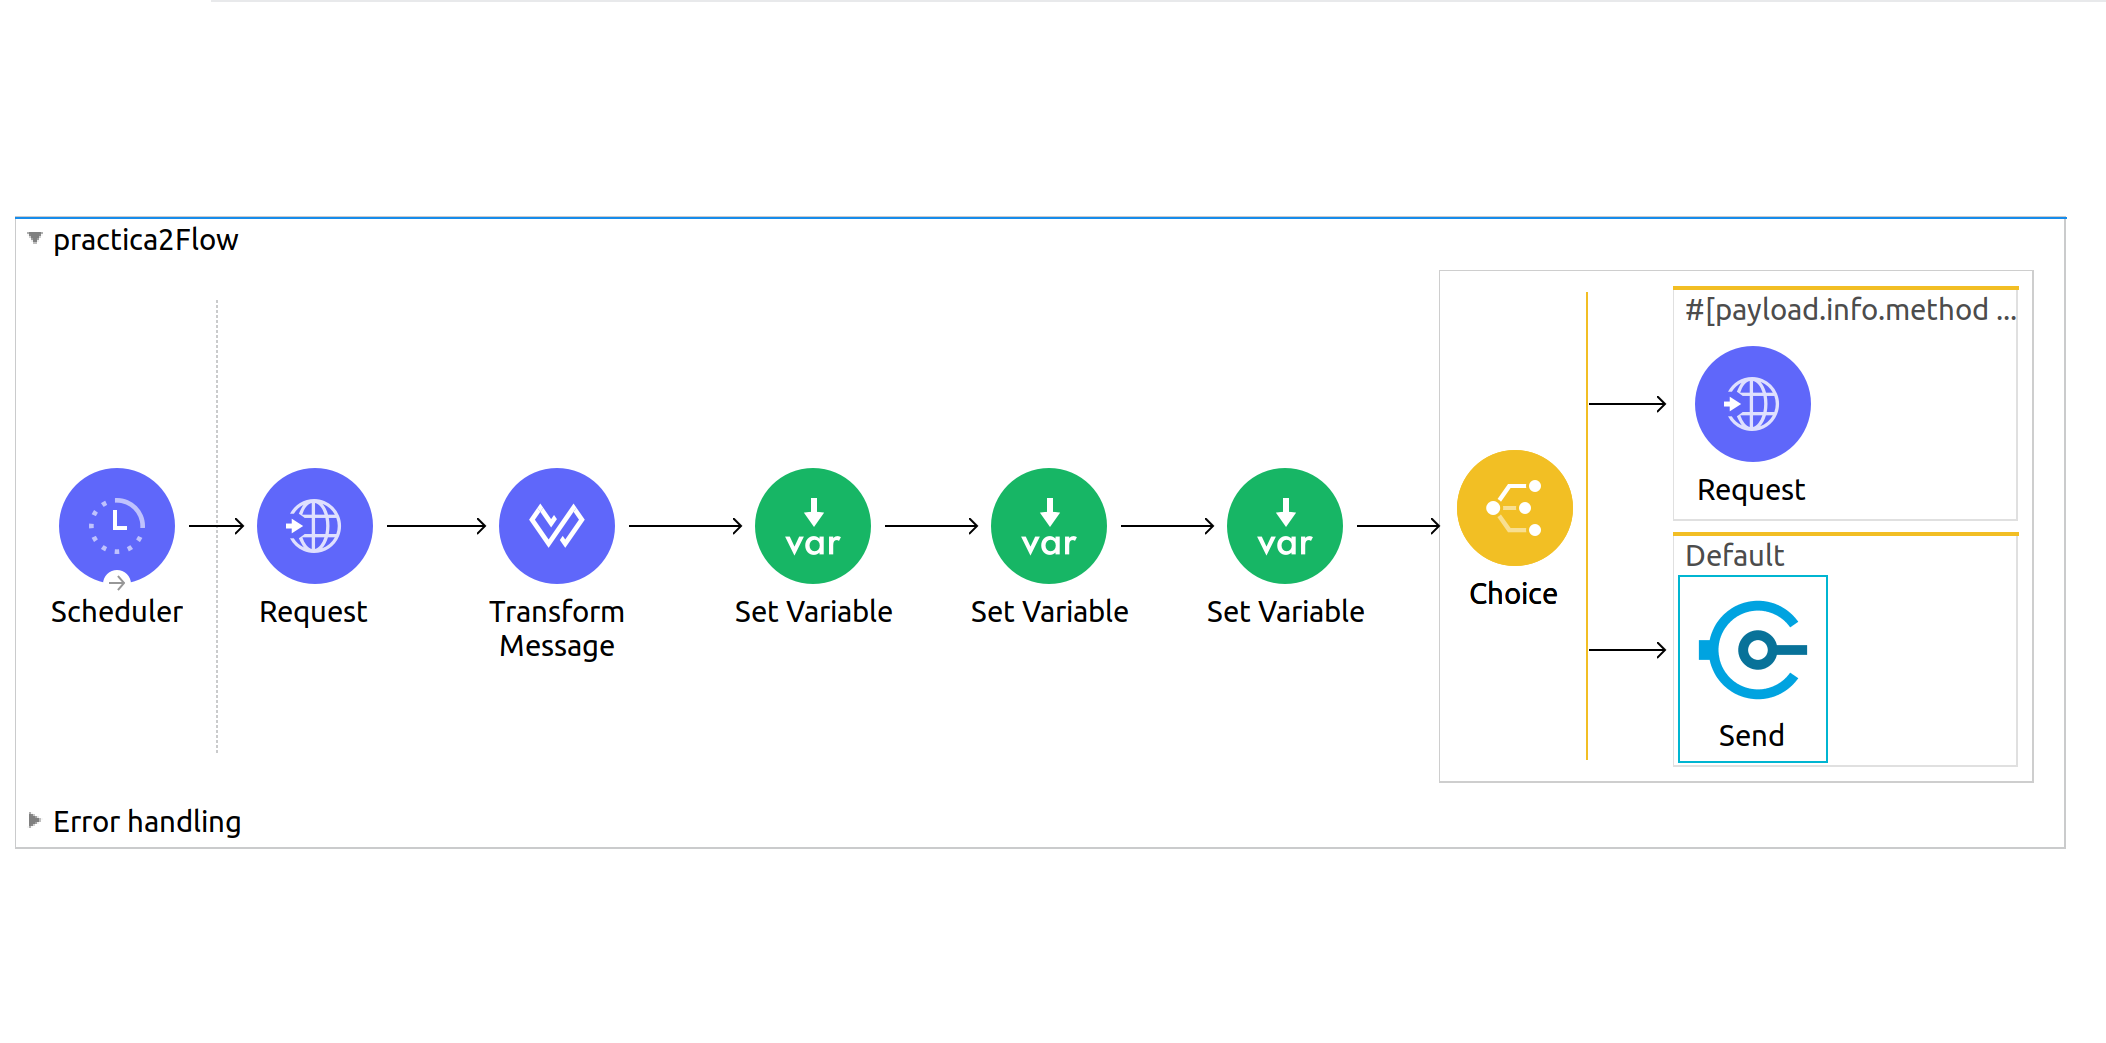
\includegraphics[width=0.7\linewidth]{./mule}
\caption{Flow final de la práctica de mule}
\end{figure}
\\
Por último, detallare brevemente cada paso a seguir para cada etapa del flow final.\\

\begin{enumerate}
    \item \underline{Scheduler}: Se crea un scheduler para poder ejecutar el flow cada cierto periodo. Con esto
          ya no dependo de entradas de información externas.
    \item \underline{Request}: Se crea una request a mi servidor local que obtiene la informacion sobre un email
          y lo que debe hacer con el, si volver a hacer un peticion al servidor local y enviar un email.
    \item \underline{Transform Message}: Lo utilizo principalmente para convertir la cadena del servidor en un objeto
          propiamente, con todos sus atributos publicos.
    \item \underline{Set Variable (x3)}: Se crean 3 instancias de Set Variable para obtner la informacion del payload e
          introducirlas como variables del flow. Esto es así, porque en el Choice posterior, solo permite
          añadir información dinámica, usando las expresiones del tipo `\#[vars.x]', donde \[ x \in V \] y
          `V' es el conjunto de variables.
    \item \underline{Choice}: Una vez llegamos a este punto, comprobamos si el método de manipular la informacion es igual
          a `db' o a `mail'. En caso de ser el primero, hacemos una request nuevamente a nuestro servidor local
          y con el parametros GET `save\_to\_db' con el valor del email previamente solicitado. En caso de ser el
          segundo, se enviara un email automatico con un correo origen y otro destino. Es importante matizar que
          todo esta puesto para que se obtenga la información de forma dinámica, es decir, el correo origen,
          el correo destino y la clave de aplicación, se obtiene todo del servidor (archivo index.php adjuntado
          en la practica).
    \item El ciclo de vuelve a repetir una vez por segundo, como indica el Scheduler detallado en el primer paso.
\end{enumerate}

\end{document}
